\chapter{Full GPyTorch Code Examples}

The following are code examples for training and evaluating GPyTorch models.\footnote{
  Tested against GPyTorch v1.1---\gp{TODO: url}.
}
We include examples for a standard GP (with no approximations/exploitable structure) and a multitask GP.
Both models can be modified to use scalable methods by changing the {\tt covar\_module} (i.e. kernel).



\section{Standard GP Regression}
\label{app:standard_gp_example}

Here we train a standard GP with a {\tt RBFKernel}.
As described in \cref{sec:programmability}, each kernel object outputs a {\tt LazyTensor} object, which defines its own {\tt \_matmul($\cdot$)} function.
If the kernel has exploitable structure---e.g.
%
\begin{itemize}
  \item {\tt LinearKernel} for Bayesian linear regression,
  \item {\tt GridInterpolationKernel} wrapping a {\tt RBFKernel} for KISS-GP,
\end{itemize}
%
then the kernel will output the appropriate {\tt LazyTensor} subclass with a structure-exploiting {\tt \_matmul($\cdot$)} function for use with the mBCG algorithm.

\longcodetrue
\begin{minted}{python3}
import math
import torch
import gpytorch
from matplotlib import pyplot as plt

"""
Training data is 100 points in [0,1] inclusive regularly spaced
True function is sin(2*pi*x) with Gaussian noise
"""
train_x = torch.linspace(0, 1, 100)
train_y = torch.sin(train_x * (2 * math.pi)) + \
    torch.randn(train_x.size()) * math.sqrt(0.04)

"""
Now we define a class for basic GP models
"""
class ExactGPModel(gpytorch.models.ExactGP):
    def __init__(self, train_x, train_y, likelihood):
        super(ExactGPModel, self).__init__(
            train_x, train_y, likelihood
        )
        self.mean_module = gpytorch.means.ZeroMean()
        # We can implement specialty models by replacing
        # this kernel (e.g. LinearKernel.)
        # Each kernel uses a differen LazyTensor under the hood.
        self.covar_module = gpytorch.kernels.ScaleKernel(
            gpytorch.kernels.RBFKernel()
        )
        # To implement KISS-GP, wrap this kernel inside al
        # gpytorch.kernels.GridInterpolationKernel

    def forward(self, x):
        mean_x = self.mean_module(x)
        # Our kernel module returns a NonLazyTensor object.
        # If we were to replace it with a LinearKernel,
        # the output would be a RootLazyTensor
        covar_x = self.covar_module(x)
        return gpytorch.distributions.MultivariateNormal(
            mean_x, covar_x
        )

"""
Create an instance of our model and likelihood
"""
likelihood = gpytorch.likelihoods.GaussianLikelihood()
model = ExactGPModel(train_x, train_y, likelihood)

"""
A basic training loop.
The GPyTorch objects in this loop use BBMM under the hood.
"""
optimizer = torch.optim.Adam(model.parameters(), lr=0.01)

# "Loss" for GPs - the marginal log likelihood
# Calling this funcition uses BBMM to compute the marginal log
# likelihood and its derivative
mll = gpytorch.mlls.ExactMarginalLogLikelihood(likelihood, model)

# Training loop
model.train()
for i in range(100):
    optimizer.zero_grad()
    loss = -mll(model(train_x), train_y)
    loss.backward()
    optimizer.step()

"""
Making predictions.
We will use LOVE to for fast variances
"""
model.eval()
likelihood.eval()
# The fast_pred_var context manager turns on LOVE variances
with torch.no_grad(), gpytorch.settings.fast_pred_var():
    test_x = torch.linspace(0, 1, 51)
    pred = likelihood(model(test_x))
    # Get mean prediction
    mean = pred.mean
    # Get upper and lower confidence bounds
    lower, upper = pred.confidence_region()

"""
Plotting the model fit
"""
f, ax = plt.subplots(1, 1, figsize=(4, 3))
# Plot training data as black stars
ax.plot(train_x.numpy(), train_y.numpy(), "k*")
# Plot prediction
ax.plot(test_x.numpy(), mean.numpy(), "b")
ax.fill_between(
  test_x.numpy(), lower.numpy(), upper.numpy(), alpha=0.5
)
ax.set(ylim=[-3, 3], xlabel="x",  ylabel="y")
ax.legend(["Observed Data", "Mean", "Confidence"])
f.show()
\end{minted}
\longcodefalse

\begin{figure}[h!]
  \centering
  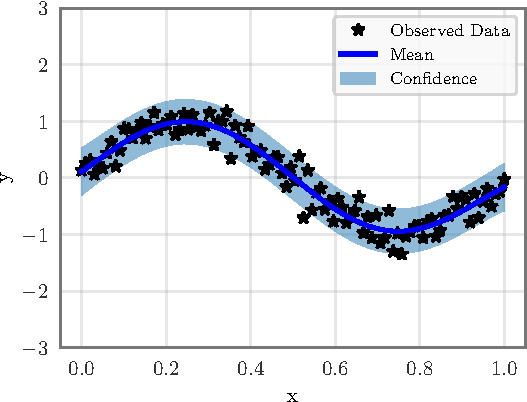
\includegraphics[width=0.5\linewidth]{figures/example_gpytorch_plot.pdf}
  \caption{
    Output plot from GPyTorch code example for standard GPs.
  }
  \label{fig:example_gpytorch_plot}
\end{figure}







\section{Multitask GP Regression}
\label{app:multitask_gp_example}

To demonstrate the modularity afforded by BBMM, we also include a code example of a multitask GP model.
What's notable is that this code example is essentially the same as the standard GP code example.
The only major difference is the kernel module ({\tt MultitaskKernel}),
which uses the ({\tt KroneckerProductLazyTensor}) under the hood for efficient inference.

\longcodetrue
\begin{minted}{python3}
import math
import torch
import gpytorch
from matplotlib import pyplot as plt

"""
Training data is 100 points in [0,1] inclusive regularly spaced
We train two outputs: a sin function and a cos function
    with Gaussian noise
"""
train_x = torch.linspace(0, 1, 100)
train_y = torch.stack([
    torch.sin(train_x * (2 * math.pi)),
    torch.cos(train_x * (2 * math.pi))
], -1)
train_y += torch.randn_like(train_y) * 0.2

"""
Now we define a class for multitask GP models
"""
class MultitaskGPModel(gpytorch.models.ExactGP):
    def __init__(self, train_x, train_y, likelihood):
        super(MultitaskGPModel, self).__init__(
            train_x, train_y, likelihood
        )
        self.mean_module = gpytorch.means.MultitaskMean(
            gpytorch.means.ZeroMean(), num_tasks=2
        )
        self.covar_module = gpytorch.kernels.MultitaskKernel(
            gpytorch.kernels.RBFKernel(), num_tasks=2, rank=1
        )

    def forward(self, x):
        mean_x = self.mean_module(x)
        covar_x = self.covar_module(x)
        return gpytorch.distributions.MultitaskMultivariateNormal(
            mean_x, covar_x
        )

"""
Create an instance of our model and likelihood
This example uses a MultitaskGaussianLikelihood to have seperate
    observation noise for each task.
"""
likelihood = gpytorch.likelihoods.MultitaskGaussianLikelihood(
    num_tasks=2
)
model = MultitaskGPModel(train_x, train_y, likelihood)


"""
Training with BBMM.
"""
optimizer = torch.optim.Adam(model.parameters(), lr=0.1)
mll = gpytorch.mlls.ExactMarginalLogLikelihood(likelihood, model)

model.train()
for i in range(100):
    optimizer.zero_grad()
    loss = -mll(model(train_x), train_y)
    loss.backward()
    optimizer.step()

"""
Making predictions with LOVE.
"""
model.eval()
likelihood.eval()
with torch.no_grad(), gpytorch.settings.fast_pred_var():
    test_x = torch.linspace(0, 1, 51)
    pred = likelihood(model(test_x))
    mean = pred.mean
    lower, upper = pred.confidence_region()


"""
Plotting the model fit
"""
f, (y1_ax, y2_ax) = plt.subplots(1, 2, figsize=(8, 3))
# Plot training data as black stars
y1_ax.plot(
    train_x.detach().numpy(), train_y[:, 0].detach().numpy(),
    "k*"
)
y2_ax.plot(
    train_x.detach().numpy(), train_y[:, 1].detach().numpy(),
    "k*"
)
# Plot predictions
y1_ax.plot(test_x.numpy(), mean[:, 0].numpy(), "b")
y2_ax.plot(test_x.numpy(), mean[:, 1].numpy(), "b")
# Shade in confidence
y1_ax.fill_between(
    test_x.numpy(), lower[:, 0].numpy(), upper[:, 0].numpy(),
    alpha=0.5
)
y2_ax.fill_between(
    test_x.numpy(), lower[:, 1].numpy(), upper[:, 1].numpy(),
    alpha=0.5
)
# Legend and axes
y1_ax.legend(["Observed Data", "Mean", "Confidence"])
y1_ax.set(ylim=[-3, 3], xlabel="x",  ylabel="y1")
y2_ax.set(ylim=[-3, 3], xlabel="x",  ylabel="y2")
f.show()
\end{minted}
\longcodefalse

\begin{figure}[h!]
  \centering
  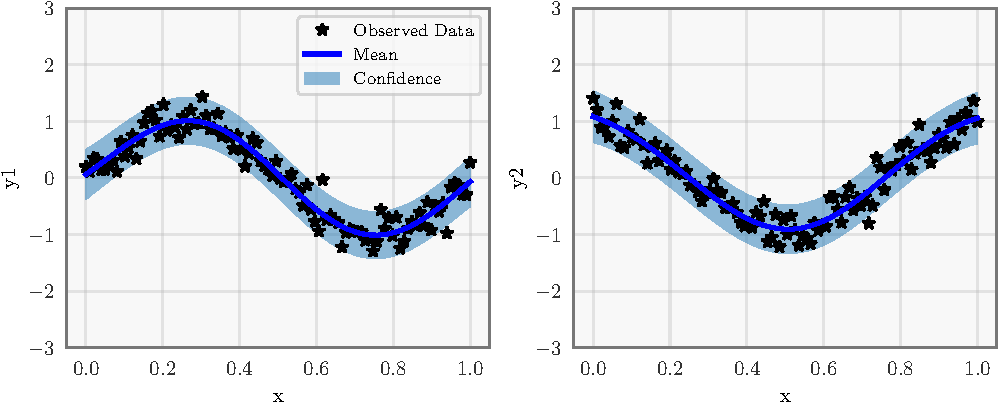
\includegraphics[width=\linewidth]{figures/example_gpytorch_plot_multitask.pdf}
  \caption{
    Output plot from GPyTorch code example for multitask GPs.
  }
  \label{fig:example_gpytorch_plot_multitask}
\end{figure}
